\section{Format d'adresse}\label{sec:archi-adresses}
\renewcommand{\rightmark}{Format d'adresse}

Cette section décrit les possibilités envisagées pour le choix du format des adresses utilisées pour les communications LoRa et motive le choix d'un format. Dans chaque hypothèse, un réseau RPL possède un préfixe de sous-réseau qui lui est propre.

\subsection*{Adresse IPv6}
    La première solution envisagée est d'utiliser les adresses IPv6 des noeuds.
    Une racine RPL peut ainsi vérifier si un paquet est destiné à son réseau et la racine LoRa à elle même,
    via le préfixe de sous réseau de l'adresse de destination.
    Cette solution est la plus simple à mettre en oeuvre car elle ne nécéssite pas de table de routage ou de processus de conversion d'adresse. Cette approche a néanmoins le désavantage que les adresses IP de 128 bits sont transportées sur un lien LoRa ce qui représente un temps de transmission important.

    Ainsi, sur l'exemple de la figure~\ref{fig:archi-topologie}, un noeud RPL du réseau ayant le préfixe $0x02$ aurait par exemple l'adresse suivante:\newline 
    \texttt{fd00::2:eeff:212:4b00:60d:611b}.
    
\subsection*{Préfixe et \textit{node-id}}
    Une seconde approche est d'utiliser un préfixe et le \textit{node-id}. Ce dernier est un identifiant de noeud sur 16 bits utilisé dans Contiki. Son calcul, basé sur les deux derniers octets de l'adresse MAC du noeud (\textit{link-layer address}) est le suivant:
    \[
        node\_id = link\_addr[s-1] + (link\_addr[size -2] << 8)
    \]
    où $s$ est la taille de la \textit{link-layer address}.\\

    Le format d'adresse utilisé serait alors un préfixe sur 8 bits et le \textit{node-id} sur 16 bits ce qui fait un total de 24 bits.

    L'avantage de cette solution est que la taille des adresses est réduite d'un facteur de 18,75\%. Néanmoins, un processus de conversion est nécessaire ainsi qu'une table de conversion d'un \textit{node-id} vers une adresse MAC pour chaque noeud RPL. En effet, le calcul du \textit{node-id} ne permet pas de reconstituer l'adresse MAC de 64 bits à partir de celui-ci.
    Un autre inconvénient est que l'utilisation du préfixe de 8 bits limite le nombre de réseaux RPL à 256, ce qui reste néanmoins acceptable.

    Ainsi, sur l'exemple de la figure~\ref{fig:archi-topologie}, un noeud RPL dont la valeur du \textit{node-id} est 24859, appartenant au réseau ayant le préfixe $0x02$, aurait par exemple l'adresse suivante: \texttt{2:24859}.

    % === infos ===
    % Dans contiki, la link layer address est "remplie" dans arch/zoul/platform.c par
    % `ieee_addr_cpy_to(linkaddr_node_addr.u8, LINKADDR_SIZE);` qui est définie dans
    % arch/cpu/cc2538/iee-addr.c qui va lire l'adresse dans la mémoire flash du cc2538
    % sauf si IEEE_ADDR_CONF_HARDCODED est définie. Dans ce cas c'est une adresse harcodée
    % qui est utilisée
    %

\subsection*{Préfixe et adresse MAC}
    La troisième approche envisagée a pour objectif de résoudre le problème de la conversion \textit{node-id} $\leftrightarrow	$ adresse MAC, en remplaçant le \textit{node-id} par l'adresse MAC d'un noeud.

    Cette solution permet une conversion d'adresse simple et la taille des adresses est de 72 bits (64 bits de l'adresse MAC et 8 bits du préfixe).

    Ainsi, sur l'exemple de la figure~\ref{fig:archi-topologie}, un noeud RPL dont l'adresse MAC est \texttt{0012.4b00.060d.611b}, appartenant au réseau ayant le préfixe $0x02$, aurait par exemple l'adresse suivante: \texttt{2:0012.4b00.060d.611b}.

\subsection*{Solution retenue}
    La solution retenue est l'utilisation du préfixe de 8 bits et du \textit{node-id} car c'est la solution qui offre les adresses les plus courtes.    
    Pour éviter l'utilisation d'une table de conversion \textit{node-id}$\leftrightarrow$ adresse MAC, une meilleure solution est d'utiliser les adresses MAC des noeuds et de modifier les 6 premiers octets de cette dernière. Cela permet de reconstituer une adresse IPv6 simplement, mais cela réduit le nombre d'adresses possibles qui reste cependant largement suffisant pour ce projet.

    Plus précisement, les adresses IPv6 seront construites tel qu'illustré par la figure~\ref{fig:archi-address}.

    \begin{figure}[H]
        \centering
        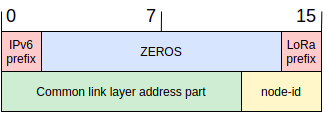
\includegraphics[scale=0.4]{res/pictures/loraaddr-ipv6.drawio.png}
        \caption{Format d'adresse IPv6 à partir d'une adresse LoRaMAC.}
        \label{fig:archi-address}
    \end{figure}
    
    Le préfixe IPv6 choisi est celui des adresses IPv6 unique local unicast. Ce type d'adresse est spécifié par le RFC 4193~\cite{rfc4193}. Car, comme indiqué dans le RFC, ces adresses sont destinées à des communications locales et sont destinées à être routées dans un réseau limité, ce qui correspond à notre réseau. Comme défini par le RFC, le préfixe IPv6 est donc \texttt{FC00::/7} suivi d'un bit à 1 qui est destiné à une utilisation future. Les adresses commencent donc par \texttt{FD}.

    Ce préfixe est suivi de 6 octets de zéros, du préfixe LoRa sur 1 octet, de la partie commune de l'adresse MAC sur 6 octets et finalement du \textit{node-id} du noeud.

    L'adresse de l'interface LoRa de la racine LoRa est quand à elle configurée administrativement.